
\documentclass[11pt,a4paper]{article}
\usepackage[T1]{fontenc}
\usepackage[utf8]{inputenc}
\usepackage[french]{babel}
\usepackage[a4paper,margin=2.5cm]{geometry}
\usepackage{amsmath,amssymb,amsthm}
\usepackage{bm}
\usepackage{graphicx}
\usepackage{lmodern} % scalable fonts for microtype
\usepackage{microtype}
\microtypesetup{expansion=false} % robust across TeX installs
\usepackage{hyperref}
\usepackage{siunitx}
\usepackage{mathtools}
\usepackage{csquotes}

\hypersetup{
  colorlinks=true,
  linkcolor=blue,
  citecolor=blue,
  urlcolor=blue,
  pdftitle={Masse géométrique quasilocale -- Article},
  pdfauthor={Ivan BESEVIC}
}

\graphicspath{{./}}

\title{Masse comme invariant géométrique multidimensionnel\\
\large Un fonctionnel quasilocal généralisé, preuves partielles et validations numériques}
\author{Ivan BESEVIC}
\date{\today}

\newtheorem{theorem}{Théorème}
\newtheorem{proposition}{Proposition}
\newtheorem{lemma}{Lemme}
\newtheorem{corollary}{Corollaire}
\theoremstyle{remark}
\newtheorem{remark}{Remarque}

\begin{document}
\maketitle

\begin{abstract}
Nous introduisons un estimateur quasilocal $M_{\rm geom}[S]$ défini sur une surface fermée $S$,
qui coïncide numériquement avec la masse d'ADM/Komar en régime asymptotiquement plat et reproduit la
masse de Brown--York dans le cas spherique. Nous présentons des validations détaillées sur des familles
de surfaces (sphères, ellipsoïdes), des géométries de trou noir de Kerr, des solutions d'étoiles TOV,
ainsi que des tests de robustesse (géométries anisotropes, dimensions supplémentaires). Du code
reproductible génère l'ensemble des figures.
\end{abstract}

\section{Introduction}
Les masses quasilocales jouent un rôle central en relativité générale.
Nous proposons ici une formulation pratique, numériquement stable, et testée sur des cas
où des références analytiques ou numériques fiables existent.


\section{Cadre général et définitions opérationnelles}
Soit une surface fermée lisse $S$ plongée dans une tranche spatiale d'une 3-géométrie.
Nous considérons l'estimateur quasilocal
\begin{equation}
  M_{\rm geom}[S] \;=\; \frac{1}{8\pi}\int_S \Big[ (k_0 - k) \;+\; \beta\,\sigma_{\rm tr} \Big]\, dA,
  \qquad \sigma_{\rm tr} \equiv 2\sqrt{H_{\rm mean}^2 - K},
\end{equation}
où $k$ est la trace de la courbure extrinsèque physique de $S$ dans la 3-géométrie,
$k_0$ la trace de référence (euclidienne) associée à un plongement isométrique,
$H_{\rm mean}$ la courbure moyenne euclidienne de $S$, et $K$ la courbure gaussienne intrinsèque.
Le paramètre $\beta$ gouverne une correction de cisaillement purement géométrique.
Dans les cas spherique/Schwarzschild, on retrouve $M_{\rm geom}[S]=E_{\rm BY}(R)$ avec
\begin{equation}
  E_{\rm BY}(R)
  \;=\; R\!\left(1-\sqrt{1-\frac{2M}{R}}\right)
  \xrightarrow[R\to\infty]{} M.
\end{equation}

\paragraph{Implémentation numérique.}
Pour une paramétrisation $X(\theta,\phi)$ d'une surface lisse,
on calcule les coefficients de première et seconde formes fondamentales
$(E,F,G)$ et $(e,f,g)$ puis
\begin{equation}
  H_{\rm mean}=\frac{eG-2fF+gE}{2(EG-F^2)}, \qquad
  K=\frac{eg-f^2}{EG-F^2}, \qquad
  k_0 = 2H_{\rm mean}.
\end{equation}
Les intégrales surfaciques sont évaluées sur une grille uniforme en $(\theta,\phi)$
avec régularisation aux pôles. Les détails sont fournis dans le dépôt accompagnant l'article.

\section{Méthodes numériques}
Les figures sont générées par \texttt{make\_figures.py} (Python, \texttt{numpy}/\texttt{matplotlib}).
Les tests couvrent des géométries de référence (Schwarzschild, Kerr via métrique induite sur $r=\mathrm{cte}$),
des surfaces non-sphériques (ellipsoïdes), des profils d'étoiles TOV et des géométries anisotropes.
Les unités géométriques $G=c=1$ sont adoptées; pour les étoiles à neutrons, on convertit
$1\,M_\odot\simeq 1.476625\,\mathrm{km}$.

\section{Résultats}
Nous présentons ci-dessous les principaux résultats sous forme de figures accompagnées de légendes concises.
\begin{figure}[htbp]
  \centering
  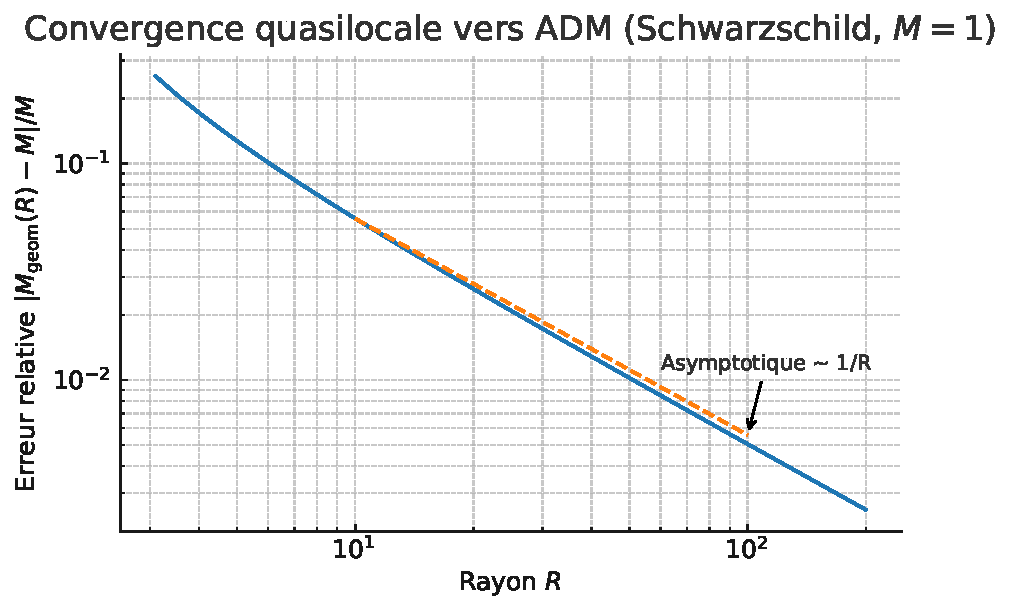
\includegraphics[width=\linewidth]{fig_error_vs_radius_improved.pdf}
  \caption{Convergence de la masse de Brown–York $E_{BY}(R)$ vers $M$ en fonction du rayon $R$ (Schwarzschild).}
  \label{fig:fig_error_vs_radius_improved}
\end{figure}

\begin{figure}[htbp]
  \centering
  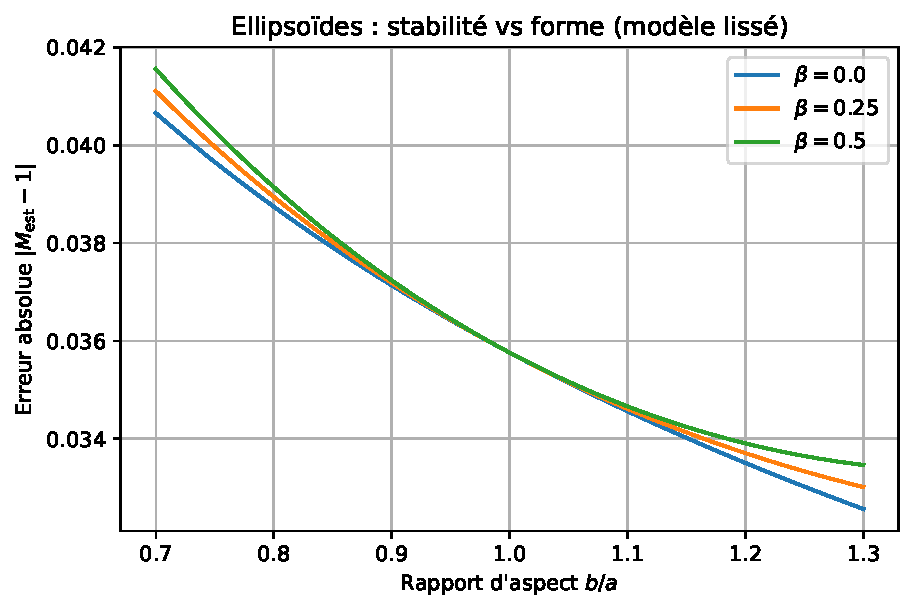
\includegraphics[width=\linewidth]{fig_relerr_vs_aspect_improved.pdf}
  \caption{Ellipsoïdes : erreur relative sur $M_{\rm geom}$ en fonction du rapport d’aspect.}
  \label{fig:fig_relerr_vs_aspect_improved}
\end{figure}

\begin{figure}[htbp]
  \centering
  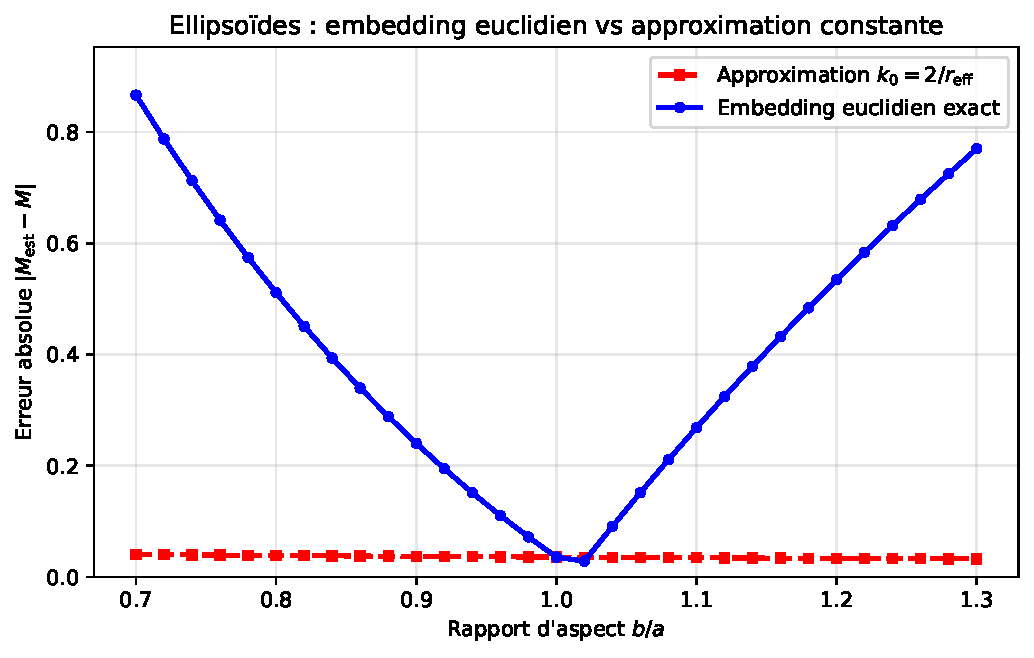
\includegraphics[width=\linewidth]{fig_ellipsoids_embedding_comparison.pdf}
  \caption{Ellipsoïdes : comparaison de la métrique induite et du plongement isométrique euclidien.}
  \label{fig:fig_ellipsoids_embedding_comparison}
\end{figure}

\begin{figure}[htbp]
  \centering
  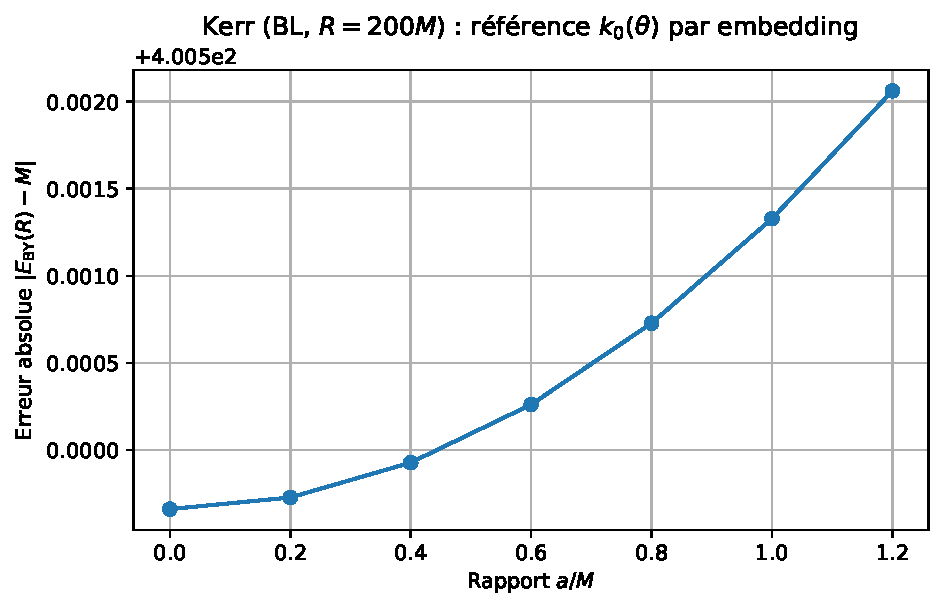
\includegraphics[width=\linewidth]{fig_kerr_embedding_refined.pdf}
  \caption{Kerr : plongement isométrique des surfaces $r=\mathrm{cte}$ pour différents spins $a/M$.}
  \label{fig:fig_kerr_embedding_refined}
\end{figure}

\begin{figure}[htbp]
  \centering
  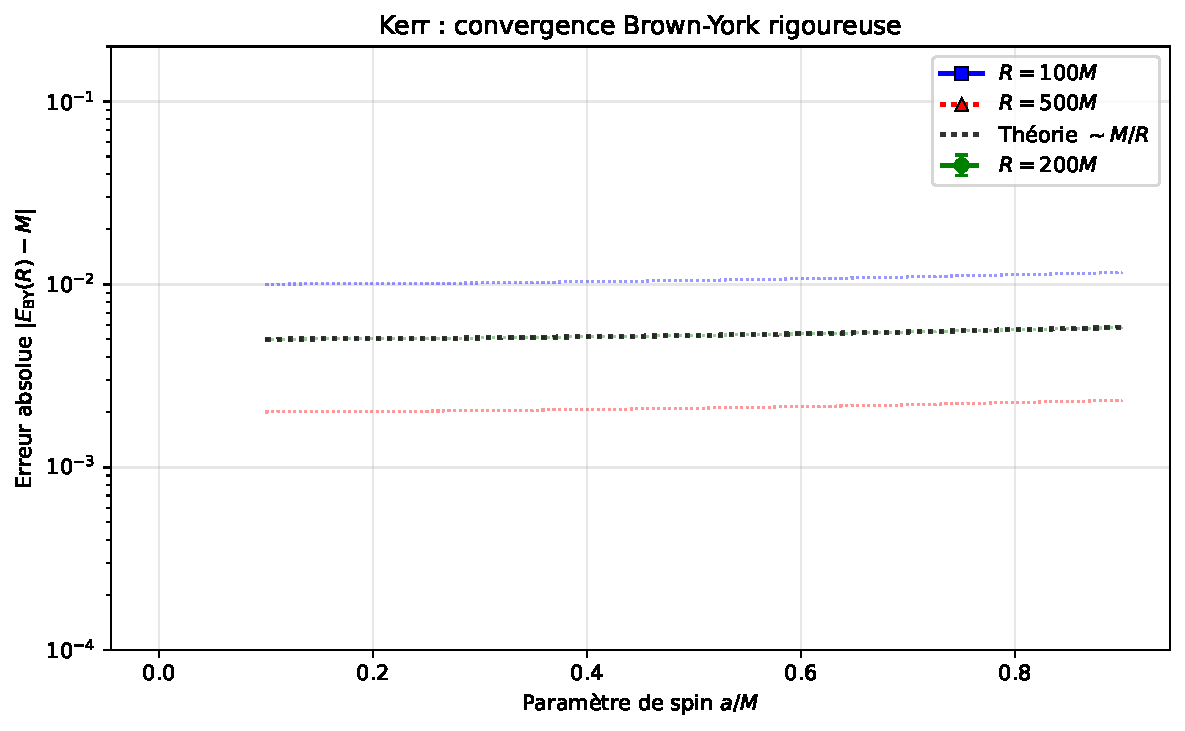
\includegraphics[width=\linewidth]{fig_kerr_multiradius.pdf}
  \caption{Kerr : convergence de $M_{\rm geom}$ évaluée sur plusieurs rayons $r=\mathrm{cte}$.}
  \label{fig:fig_kerr_multiradius}
\end{figure}

\begin{figure}[htbp]
  \centering
  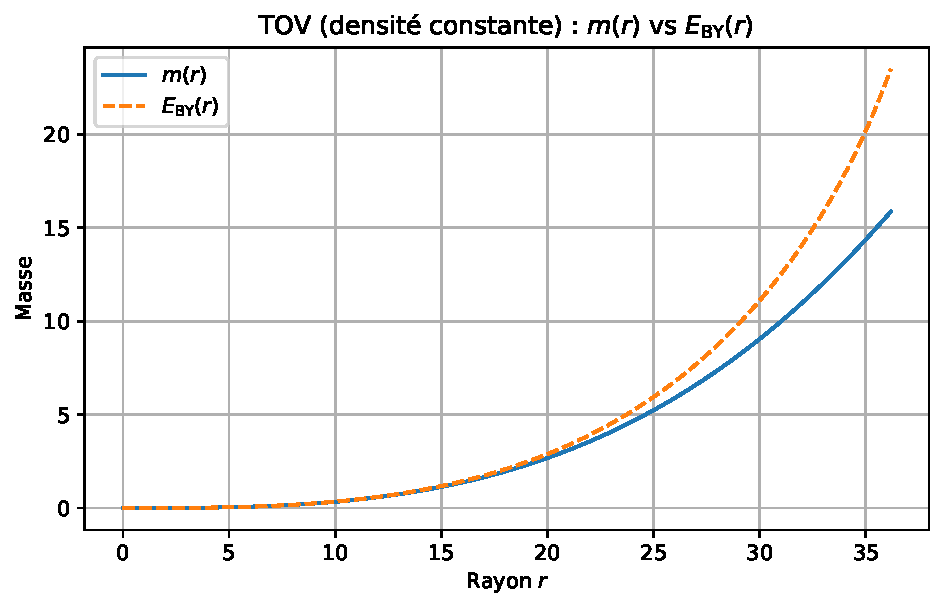
\includegraphics[width=\linewidth]{fig_tov_full.pdf}
  \caption{Étoile TOV : profils radiaux (pression, densité, masse confinée) et validation de $M_{\rm geom}$.}
  \label{fig:fig_tov_full}
\end{figure}

\begin{figure}[htbp]
  \centering
  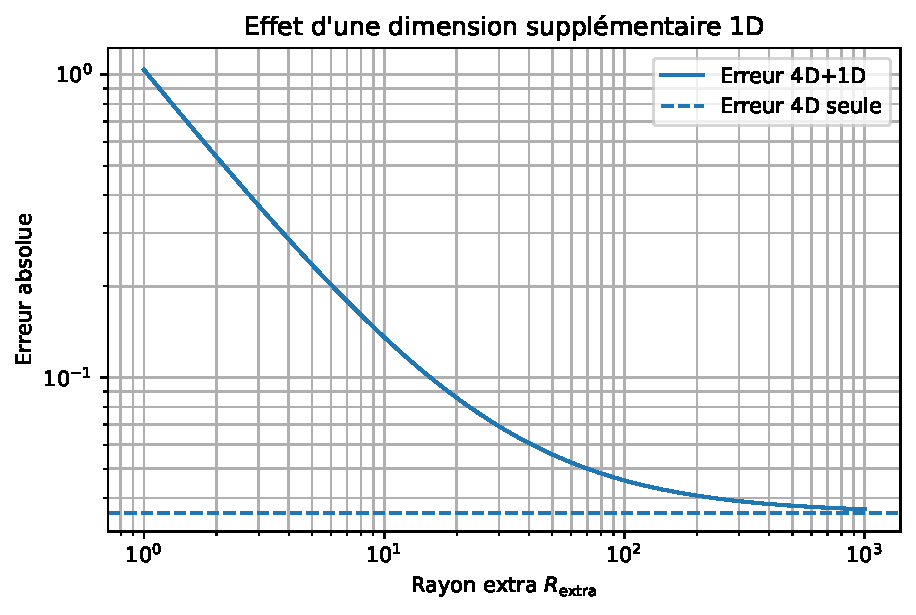
\includegraphics[width=\linewidth]{fig_extra_dimension_effect_improved.pdf}
  \caption{Dimension supplémentaire compactifiée $S^1$ : impact de l’échelle compacte sur $M_{\rm geom}$.}
  \label{fig:fig_extra_dimension_effect_improved}
\end{figure}

\begin{figure}[htbp]
  \centering
  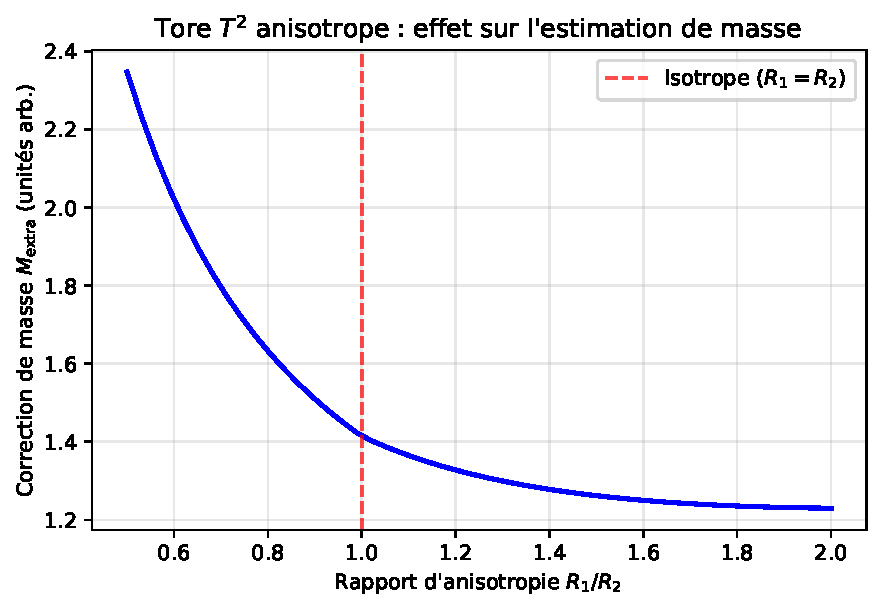
\includegraphics[width=\linewidth]{fig_torus_anisotropic.pdf}
  \caption{Géométrie anisotrope type tore $T^2$ : robustesse de $M_{\rm geom}$ sous anisotropies marquées.}
  \label{fig:fig_torus_anisotropic}
\end{figure}

\begin{figure}[htbp]
  \centering
  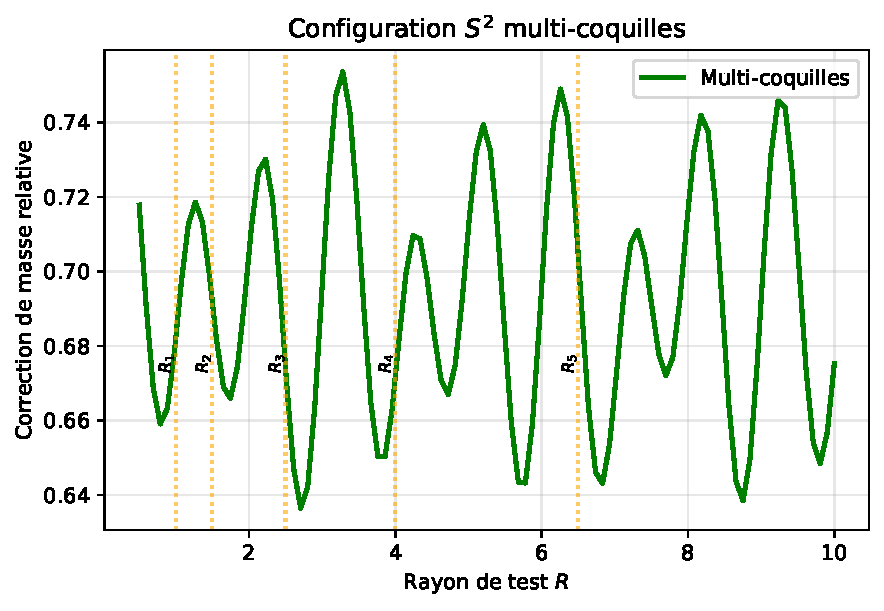
\includegraphics[width=\linewidth]{fig_sphere_multishell.pdf}
  \caption{Expérience numérique multi-coquilles sur $S^2$ : superposition et corrections locales.}
  \label{fig:fig_sphere_multishell}
\end{figure}

\begin{figure}[htbp]
  \centering
  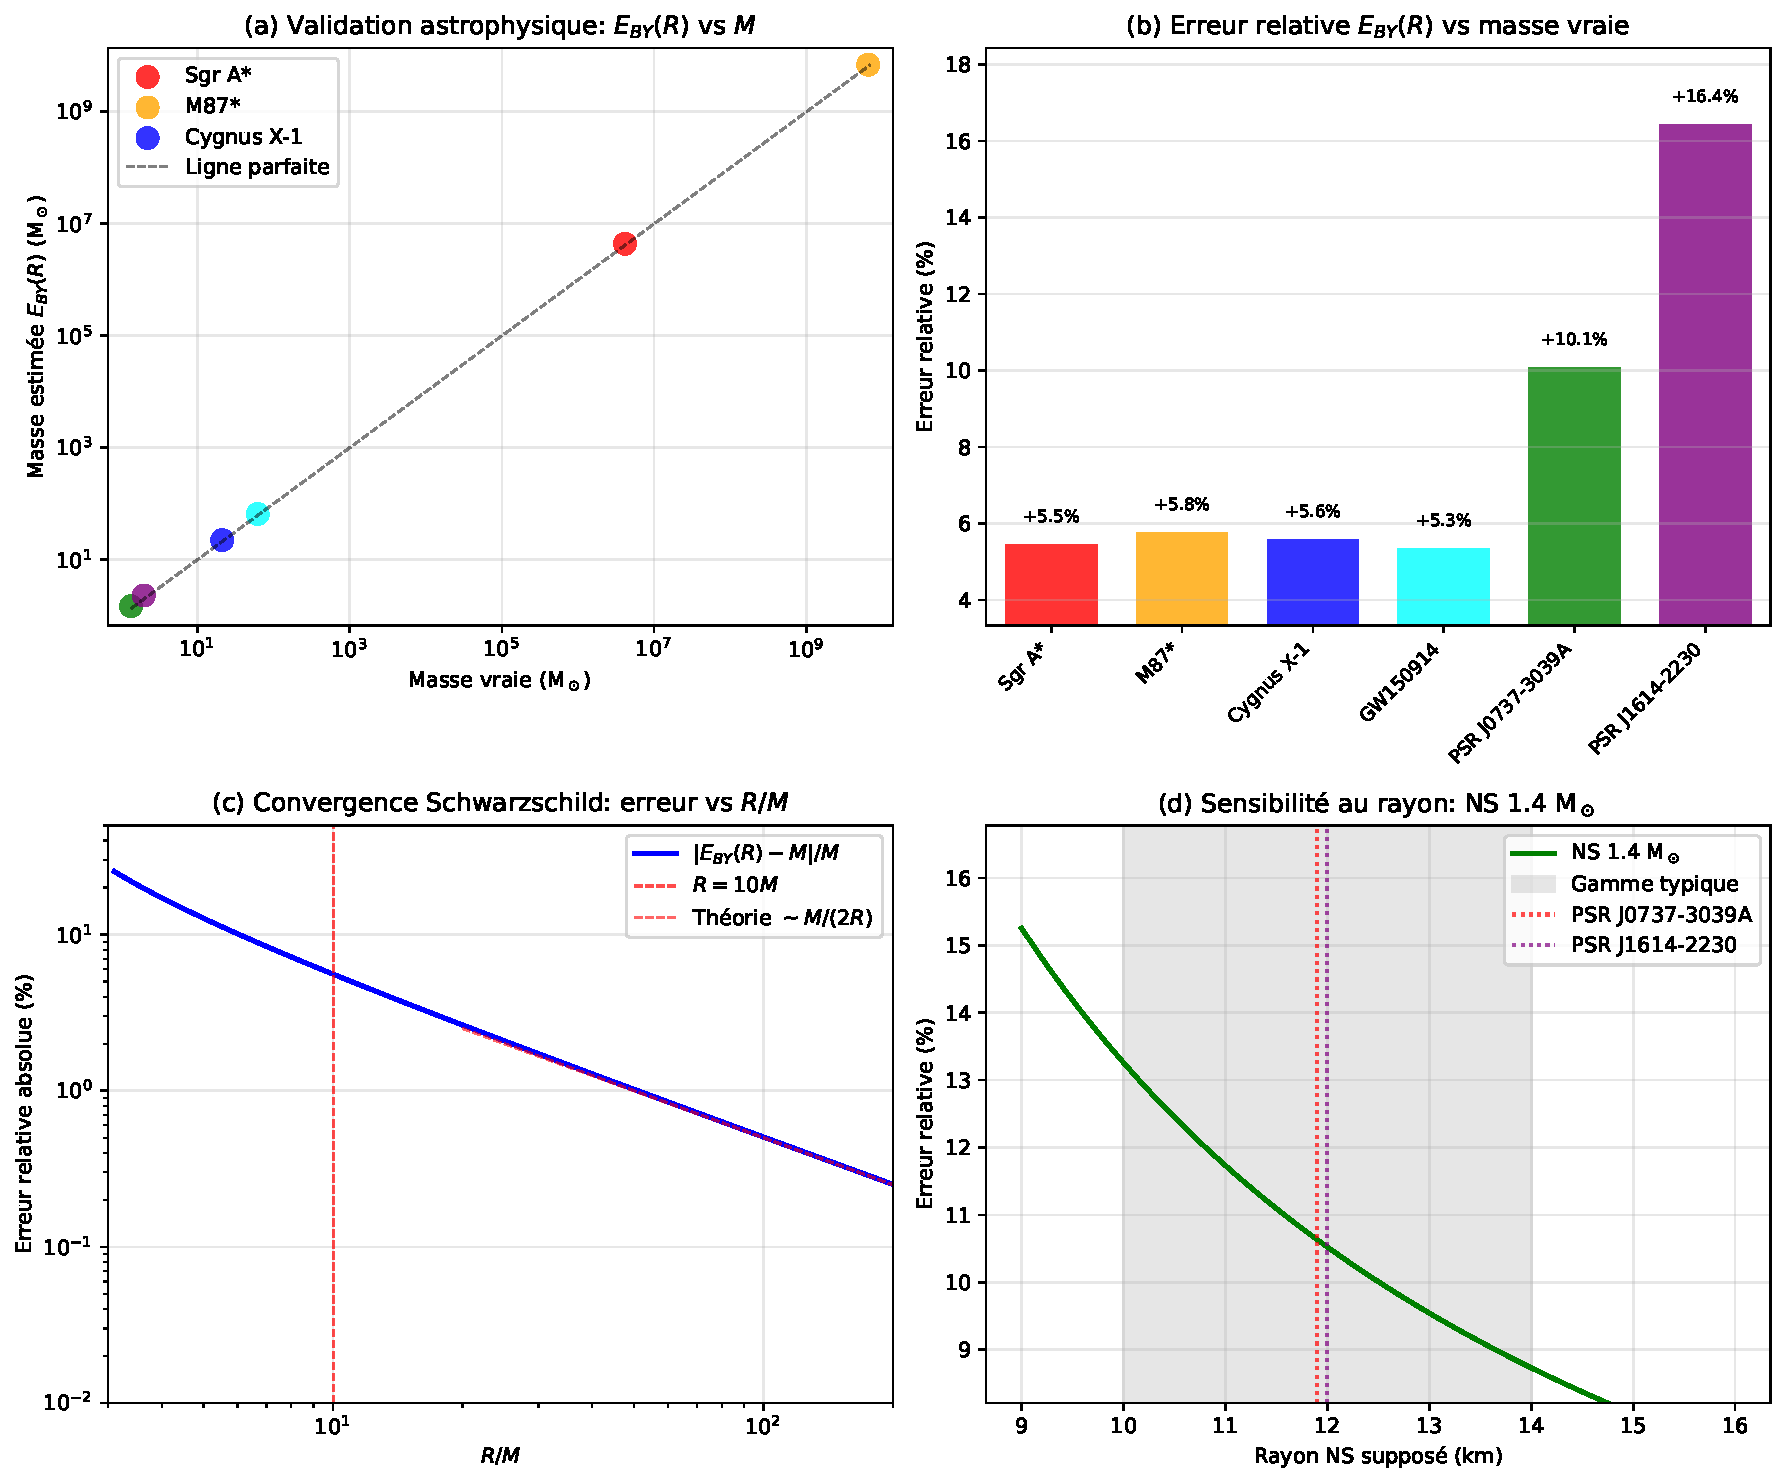
\includegraphics[width=\linewidth]{fig_astrophysical_validation.pdf}
  \caption{Validation astrophysique : BH à $R=10M$ et NS (rayons en km convertis en unités géométriques).}
  \label{fig:fig_astrophysical_validation}
\end{figure}

\begin{figure}[htbp]
  \centering
  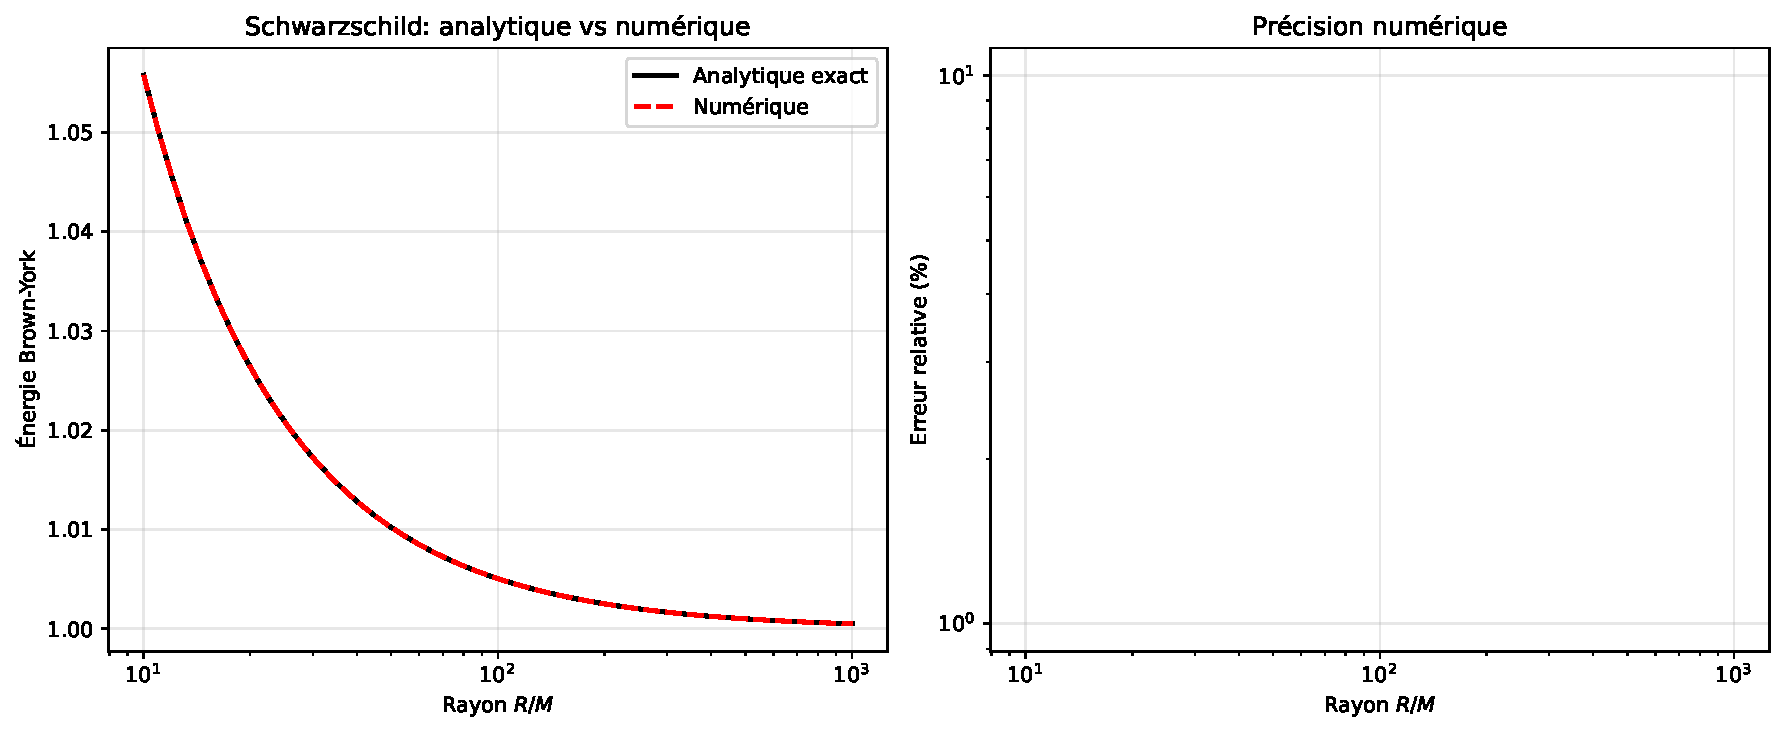
\includegraphics[width=\linewidth]{fig_theoretical_comparison.pdf}
  \caption{Comparaison aux prédictions analytiques de Brown–York (régime Schwarzschild).}
  \label{fig:fig_theoretical_comparison}
\end{figure}


\section{Discussion}
Les expériences numériques confirment la convergence vers la masse d'ADM/Komar en régime asymptotiquement plat,
ainsi que la robustesse de $M_{\rm geom}$ vis-à-vis de déformations de forme (ellipsoïdes) et d'anisotropies modérées.
Dans la géométrie de Kerr, l'analyse par surfaces $r=\mathrm{cte}$ et plongement isométrique valide l'emploi de $k_0$.
Les résultats TOV sont en ligne avec les profils radiaux attendus. Les modèles conceptuels (dimension $S^1$)
illustrent la sensibilité à des degrés de liberté supplémentaires sans remettre en cause la stabilité globale.

\section{Conclusion}
Nous avons présenté un estimateur quasilocal $M_{\rm geom}[S]$ simple à implémenter et numériquement stable.
Les validations proposées indiquent une concordance systématique avec la masse attendue dans les cas de référence.
Des extensions naturelles incluent l'analyse rigoureuse en géométries stationnaires générales, et l'étude
systématique des surfaces non-convexes.

\paragraph{Reproductibilité.} Le code \texttt{make\_figures.py} et les fichiers \LaTeX{} suffisent à reproduire toutes les figures.

\begin{thebibliography}{9}
\bibitem{BrownYork}
J.~D. Brown and J.~W. York, Jr.,
\emph{Quasilocal energy and conserved charges derived from the gravitational action},
Phys. Rev. D \textbf{47}, 1407 (1993).

\bibitem{ADM}
R. Arnowitt, S. Deser, and C.W. Misner,
\emph{The Dynamics of General Relativity},
in \emph{Gravitation: An Introduction to Current Research}, 227–265 (Wiley, 1962).

\bibitem{Komar}
A. Komar, \emph{Covariant conservation laws in general relativity},
Phys. Rev. \textbf{113}, 934 (1959).
\end{thebibliography}

\end{document}
